% ---------------------------------------------------
% CAPÍTULO
% ---------------------------------------------------
\chapter{Introdução ao modelo \textit{Notas de Aulas} em \LaTeX}

Aqui estão alguns exemplos de estruturas pré-definidas do \LaTeX\ ou criadas por mim para melhorar a organização. Para visualizar a escrita do código em latex, acesse o arquivo \verb|00_Introducao_ao_template.tex|.


% ---------------------------------------------------
% SEÇÃO
% ---------------------------------------------------
\section{Texto}

\subsection{Texto colorido}

{\textcolor{OliveGreen}{Lorem ipsum dolor em \texttt{OliveGreen}}}

{\textcolor{Red}{Lorem ipsum dolor em \texttt{Red}}}

{\textcolor{Blue}{Lorem ipsum dolor em \texttt{Blue}}}


% ---------------------------------------------------
\subsection{Listas numeradas}

Lorem ipsum dolor sit amet, consectetur adipiscing elit:
\begin{enumerate}
    \item Lorem ipsum dolor sit amet.
    \item Lorem ipsum dolor sit amet.
\end{enumerate}


% ---------------------------------------------------
\subsection{Listas ecom marcadores}

Lorem ipsum dolor sit amet, consectetur adipiscing elit:
\begin{itemize}
    \item Lorem ipsum dolor sit amet.
    \item Lorem ipsum dolor sit amet.
\end{itemize}


% \newpage


% ---------------------------------------------------
% SEÇÃO
% ---------------------------------------------------
\section{Ambientes matemáticos}

\begin{itemize}
    \item Exemplo de ambiente \texttt{equation} (equações numeradas automaticamente):
\end{itemize}
\begin{equation}
    \lim_{n\to \infty} \sum_{i=1}^{n} f(x_i)\,\Delta x 
    = \int_{a}^{b} f(x)\,dx = F(b) - F(a)
\end{equation}


\begin{itemize}
    \item Equação em exibição sem numeração:
\end{itemize}
\[
\nabla \cdot \vec{E} = \frac{\rho}{\varepsilon_0}
\]

\begin{itemize}
    \item Equações que precisam ficar alinhadas no "=", por exemplo:
\end{itemize}

Equações de Navier-Stokes Forma expandida (3D):
\begin{align*}
    \rho\left(\frac{\partial u}{\partial t} + u\frac{\partial u}{\partial x} + v\frac{\partial u}{\partial y} + w\frac{\partial u}{\partial z}\right) &= -\frac{\partial p}{\partial x} + \mu\left(\frac{\partial^2 u}{\partial x^2} + \frac{\partial^2 u}{\partial y^2} + \frac{\partial^2 u}{\partial z^2}\right) + f_x \\[0.3cm]
    \rho\left(\frac{\partial v}{\partial t} + u\frac{\partial v}{\partial x} + v\frac{\partial v}{\partial y} + w\frac{\partial v}{\partial z}\right) &= -\frac{\partial p}{\partial y} + \mu\left(\frac{\partial^2 v}{\partial x^2} + \frac{\partial^2 v}{\partial y^2} + \frac{\partial^2 v}{\partial z^2}\right) + f_y \\[0.3cm]
    \rho\left(\frac{\partial w}{\partial t} + u\frac{\partial w}{\partial x} + v\frac{\partial w}{\partial y} + w\frac{\partial w}{\partial z}\right) &= -\frac{\partial p}{\partial z} + \mu\left(\frac{\partial^2 w}{\partial x^2} + \frac{\partial^2 w}{\partial y^2} + \frac{\partial^2 w}{\partial z^2}\right) + f_z
\end{align*}
onde $\mathbf{v} = (u,v,w)$ é o campo de velocidade, $p$ é a pressão, $\rho$ é a densidade, $\mu$ é a viscosidade dinâmica e $\mathbf{f}$ representa forças externas.

\begin{itemize}
    \item Texto de exemplo com equação em linha: \( E = mc^2 \) ou também $a^2 + b^2 = c^2$.
\end{itemize}

\begin{itemize}
    \item Equação dentro de uma caixa:
\end{itemize}
\begin{equation}
    \boxed{ \nabla f(x,y,z) = \lambda\ \nabla g(x,y,z) }
\end{equation}



% \newpage


% ---------------------------------------------------
% SEÇÃO
% ---------------------------------------------------
\section{Códigos de programação}

% Exemplos com o pacote minted
% (necessário compilar com -shell-escape)

Para escrever um código de programação usando o ambiente \texttt{codigo} e \texttt{minted}:

\begin{codigo}[H]
    \begin{verbatim}
\begin{codigo}[H]
\begin{minted}{<linguagem>}
<código>
\end{minted}
\caption{<legenda>}
\label{codigo:<label>}
\end{codigo}
    \end{verbatim}
    
    \caption{Código-fonte em LaTeX para gerar um bloco de código Java. Fonte: Autor.}
    \label{cod:latex-source-verbatim}
\end{codigo}

% ---------------------------------------------------
\subsection{Linguagem Java}

\begin{codigo}[H]
\begin{minted}{java}
public class Main {
    public static void main(String[] args) {
        System.out.println("Olá, mundo!");
    }
}
\end{minted}
\caption{Código em Java usando \texttt{minted}. Fonte: Autor.}
\label{cod:java}
\end{codigo}

% ---------------------------------------------------
\subsection{Linguagem C}

\begin{codigo}[H]
\begin{minted}{c}
#include <stdio.h>

int main() {
    printf("Olá, mundo!\n");
    return 0;
}
\end{minted}
\caption{Código em C usando \texttt{minted}. Fonte: Autor.}
\label{cod:c}
\end{codigo}

% ---------------------------------------------------
\subsection{Linguagem Python}

\begin{codigo}[H]
\begin{minted}{python}
def soma(a, b):
    return a + b

print("Resultado:", soma(2, 3))
\end{minted}
\caption{Código em Python usando \texttt{minted}. Fonte: Autor.}
\label{cod:python}
\end{codigo}





% ---------------------------------------------------
% SEÇÃO
% ---------------------------------------------------
\section{Figuras}


% ---------------------------------------------------
\subsection{Uma imagem}

\begin{figure}[H]
	\centering
	\includegraphics[width=0.3\linewidth]{Imagens/ufs_horizontal_positiva.png}
	\caption{Logo da Universidade Federal de Sergipe.}
	\label{fig:logo_ufs}
\end{figure}

Para referenciar uma figura, utiliza-se o comando \verb|\ref{<label>}|, onde o \texttt{<label>} foi previamente definido com \verb|\label{<label>}| dentro do ambiente da figura. No exemplo, o código \verb|Figura \ref{fig:logo_ufs}| gera a referência "Figura \ref{fig:logo_ufs}".

Exemplo: "De acordo com a Figura \ref{fig:logo_ufs}, temos que..."


% ---------------------------------------------------
\subsection{Duas imagens}

\begin{figure}[H]
    \centering
    
    \begin{subfigure}{0.3\textwidth}
        \centering
        \includegraphics[width=\linewidth]{Imagens/ufs_horizontal_positiva.png}
        \caption{}
        \label{fig:subimagem1}
    \end{subfigure}
    \hspace{1cm} % ou \hfill
    \begin{subfigure}{0.3\textwidth}
        \centering
        \includegraphics[width=\linewidth]{Imagens/DCOMP LOGO-AZUL NOVO-01.png}
        \caption{}
        \label{fig:subimagem2}
    \end{subfigure}
    
    \caption{Legenda geral para as subfiguras.}
    \label{fig:subfiguras_lado_a_lado}
\end{figure}

Também pode-se referenciar cada uma das duas imagens separadamente, como em: "Na Figura \ref{fig:subimagem1} e na Figura \ref{fig:subimagem2}", ou referenciar ela por completo: "Figura \ref{fig:subfiguras_lado_a_lado}".




% ---------------------------------------------------
% SEÇÃO
% ---------------------------------------------------
\section{Tabelas}


\begin{table}[H]
    \centering
    
    \begin{tabular}{cc}
        \toprule
        \textbf{Material}               & \textbf{Constante dielétrica \( k \)} \\
        \midrule
        Ar (1 atm)                      & 1,00054   \\
        Poliestireno                    & 2,6       \\
        Papel                           & 3,5       \\
        Óleo de transformador           & 4,5       \\
        Pirex                           & 4,7       \\
        Porcelana                       & 6,5       \\
        Água \( \SI{20}{\celsius} \)    & 80,4      \\
        Titânia \( \mathrm{TiO_2} \)    & 130       \\
        Titanato de estrôncio           & 310       \\
        \bottomrule
    \end{tabular}
    
    \caption{Propriedades de alguns dielétricos. Fonte: \cite{halliday}.}
    \label{tab:dieletricos}
\end{table}






% ---------------------------------------------------
% SEÇÃO
% ---------------------------------------------------
\section{Ambiente \texttt{blocks}}


% ---------------------------------------------------
\subsection{Texto corrido}

\begin{blocks}{Título}
    Lorem ipsum dolor sit amet, consectetuer adipiscing elit. Ut purus elit, vestibulum ut, placerat ac, adipiscing vitae, felis. Curabitur dictum gravida mauris. Nam arcu libero, nonummy eget, consectetuer id, vulputate a, magna. Donec vehicula augue eu neque.
\end{blocks}


% ---------------------------------------------------
\subsection{Teoremas}

\begin{codigo}[H]
\begin{minted}{tex}
\begin{teorema}{titulo}{label}
    <conteúdo>
\end{teorema}
%teste de comentário
\end{minted}
\caption{Código \LaTeX para ambiente \texttt{teorema}. Fonte: Autor.}
\label{cod:ambiente_teorema}
\end{codigo}

\begin{itemize}
    \item Exemplo com título
\end{itemize}
\begin{teorema}{Comprimento de curva parametrizada}{label}
Se uma curva \( C \) é descrita por equações paramétricas \( x=f(t) \) e \( y = g(t),\ \alpha \leq t \leq \beta \), onde \( f' \) e \( g' \) são contínuas em \( \left[ \alpha, \beta \right] \), então o comprimento de \( C \) é:
\[
L = \int_\alpha^\beta \sqrt{\left( \dfrac{dx}{dt} \right)^2 + \left( \dfrac{dy}{dt} \right)^2}\ dt
\]
\end{teorema}

\begin{itemize}
    \item Exemplo sem título: basta deixar o espaço \verb|{titulo}| vazio
\end{itemize}
\begin{teorema}{}{label2}
Se uma curva \( C \) é descrita por equações paramétricas \( x=f(t) \) e \( y = g(t),\ \alpha \leq t \leq \beta \), onde \( f' \) e \( g' \) são contínuas em \( \left[ \alpha, \beta \right] \), então o comprimento de \( C \) é:
\[
L = \int_\alpha^\beta \sqrt{\left( \dfrac{dx}{dt} \right)^2 + \left( \dfrac{dy}{dt} \right)^2}\ dt
\]
\end{teorema}

Para referenciar basta escrever \verb|De acordo com o Teorema \ref{teorema:<labe>}|, ficando:

De acordo com o Teorema \ref{teorema:label}




% ---------------------------------------------------
\subsection{Exemplos}

\begin{exemplo}
    Título do exemplo

    \textbf{\textit{Resolução:}}
    
    Início da resolução...\fimresolucao
\end{exemplo}






% ---------------------------------------------------
% SEÇÃO
% ---------------------------------------------------
\section{Plotagem de gráficos usando a biblioteca \texttt{tikz} e \texttt{pgfplots}}

\subsection{Função de uma variável}

\begin{figure}[H]
	\centering
	
	\begin{tikzpicture}
		\begin{axis}[
			width=9cm,
            %height=9cm,
			title={},
			%xlabel = \( x \),
			%ylabel = {\( f(x) \)},
			axis lines = middle,
			xmin=-4.5, xmax=4.5,
			ymin=-4.5, ymax=4.5,
			xtick={-4,-3,-2,-1,0,1,2,3,4},
			ytick={-4,-3,-2,-1,0,1,2,3,4},
			legend pos=north west,
			colormap/cool,			% COR
			]
			
			\addplot[		
			samples=200,
			color=red,
			domain=-2.5:2.5,
			%shader=interp,		% Habilita a interpolação de cores
			]
			{x^3 - 4*x};
			%\addlegendentry{\( x^3 - x \)}
		\end{axis}
	\end{tikzpicture}
	
	\label{fig:funcao_uma_variavel}
	\caption{Plotagem de \( f(x) = x^3 - x \).}
\end{figure}


% ---------------------------------------------------
\subsection{Funções paramétricas}

\begin{figure}[H]
	\centering
	
    \begin{tikzpicture}
        \begin{axis}[
            width=8cm,
            height=8cm,
            %x=1.0cm,
            %y=1.0cm,
            axis lines=middle,          % Eixos no centro (x=0, y=0)
            xlabel={$x$},               % Rótulo do eixo x
            ylabel={$y$},               % Rótulo do eixo y
            %title={$y^2 = x(x-3)^2$},    % Título do gráfico
            xmin=-2, xmax=6.5,
            ymin=-4.5, ymax=4.5,
            xtick={-2,-1,0,1,2,3,4,5,6},
			ytick={-4,-3,-2,-1,0,1,2,3,4},
            %grid=major,                 % Adiciona uma grade para melhor visualização
            %legend pos=north west,      % Posição da legenda
        ]
        \addplot[
            red,                    % Usa um nome de cor padrão, mais legível
            %line width=1.5pt,       % Largura de linha um pouco mais fina
            smooth,
            samples=150,            % Mais amostras para uma curva mais suave
            variable=t,
            domain=-2.2:2.2,        % Domínio otimizado para a área visível
        ]
        ({t^2}, {t^3-3*t});
        % \legend{$x=t^2$, $y=t^3-3t$} % Adiciona uma legenda à curva
        \end{axis}
    \end{tikzpicture}
    
    \label{fig:funcao_parametrica1}
	\caption{Plotagem de \( (x,y) = (t^2,\ t^3-3t), \quad -10 \leq 0 \leq 10 \).}
\end{figure}




\begin{figure}[H]
	\centering
	
	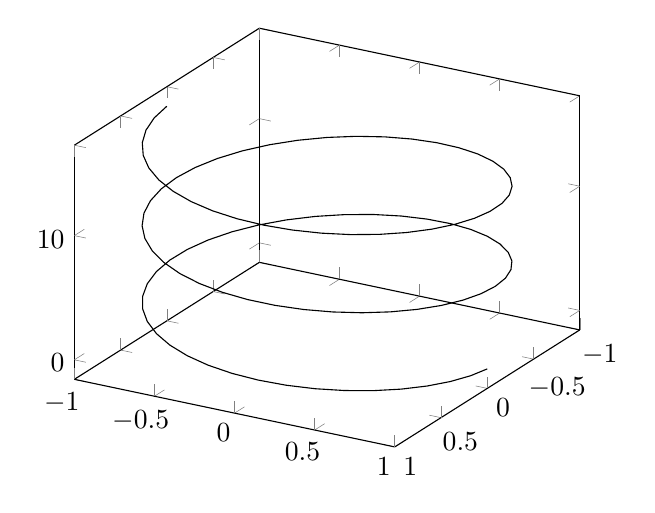
\begin{tikzpicture}
		\begin{axis}[
			width=8cm,
			title={},
			%xlabel = \( x \),
			%ylabel = {\( f(x) \)},
			%axis lines = middle,
			%xmin=-3, xmax=3,
			%ymin=-3, ymax=3,
			%xtick={-2,-1,0,1,2},
			%ytick={-2,-1,0,1,2},
			view={120}{30},
		]
		\addplot3[
			domain=0:5*pi,
			samples = 100,
			samples y=0,
		]
		({sin(deg(x))}, {cos(deg(x))}, {x});
		\end{axis}
	\end{tikzpicture}
	
	\label{fig:funcao_parametrica2}
	\caption{Plotagem de \( \langle x,y,z \rangle = \langle \sin (x),\ \cos (x),\ x \rangle \).}
\end{figure}


% ---------------------------------------------------
\subsection{Gráfico de duas variáveis}

O pacote não é muito bom para plotagem de gráficos de 2 variáveis.

\begin{figure}[H]
	\centering
	
	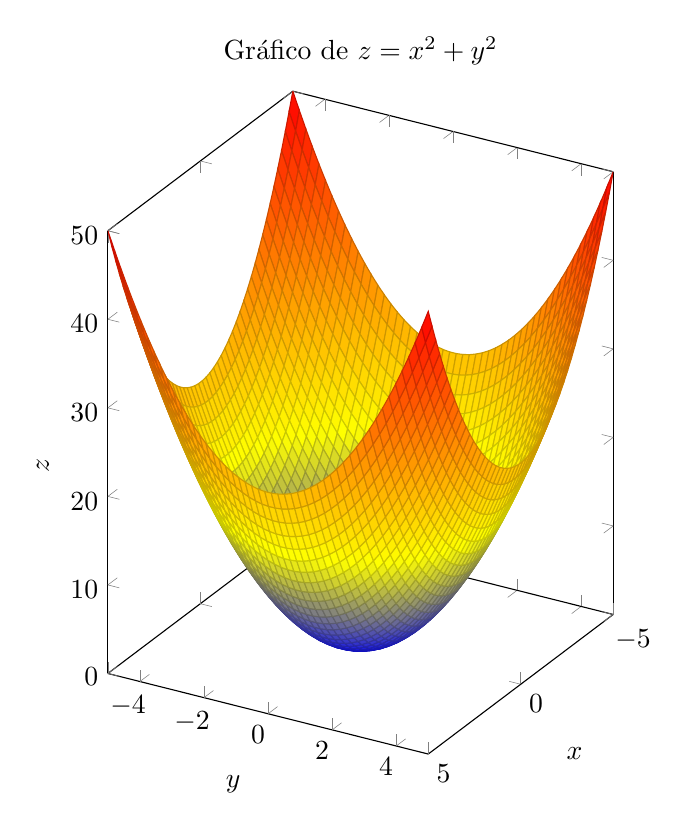
\begin{tikzpicture}
		\begin{axis}[
			height=10cm,
			width=8cm,
			title={Gráfico de \( z = x^2 + y^2 \)},
			xlabel={\(x\)},
			ylabel={\(y\)},
			zlabel={\(z\)},
			xmin=-5, xmax=5,
			ymin=-5, ymax=5,
			zmin=0, zmax=50, 			% Limites de Z ajustados
			ztick={0,10,20,30,40,50},
			view={120}{20} 				% Ajusta o ângulo de visão
			]
			\addplot3[
			surf,
			samples=50, 				% Espaço amostral
			domain=-5:5,
			]
			{x^2 + y^2};
		\end{axis}
	\end{tikzpicture}
	
	\label{fig:grafico3D}
	\caption{Plotagem de \( f(x,y) = x^2 + y^2 \).}
\end{figure}


\subsection{Malha diferenciada}

\begin{figure}[H]
	\centering
	
	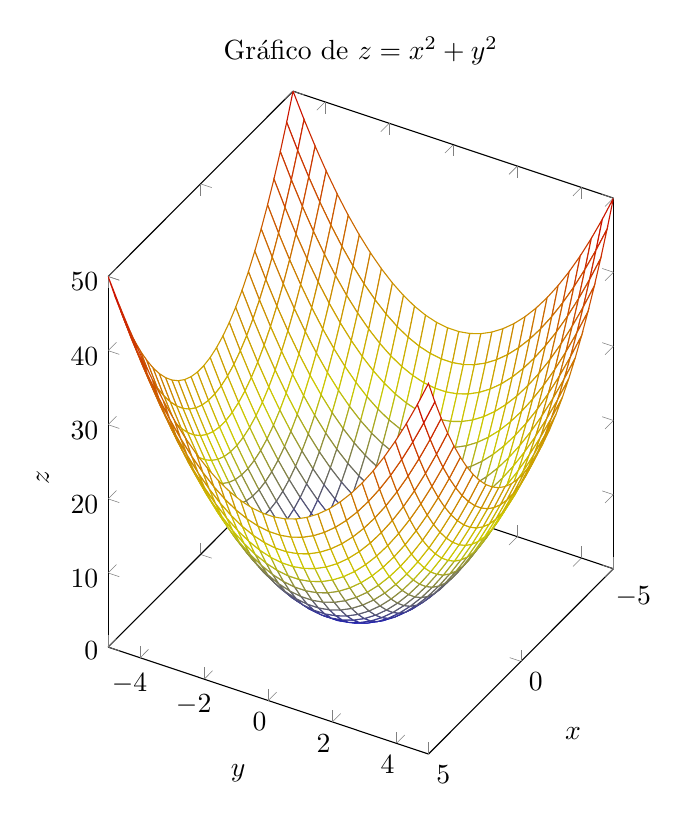
\begin{tikzpicture}
		\begin{axis}[
			height=10cm,
			width=8cm,
			title={Gráfico de \( z = x^2 + y^2 \)},
			xlabel={\(x\)},
			ylabel={\(y\)},
			zlabel={\(z\)},
			%axis lines = middle,
			xmin=-5, xmax=5,
			ymin=-5, ymax=5,
			zmin=0, zmax=50, % Limites de Z ajustados
			ztick={0,10,20,30,40,50},
			view={120}{30} % Ajusta o ângulo de visão
			]
			\addplot3[
			surf,
            fill=white,  % Adicionada esta linha para o fundo branco
			samples=30, % Menos amostras para compilar mais rápido
			domain=-5:5,
			]
			{x^2 + y^2};
		\end{axis}
	\end{tikzpicture}
	
	\label{fig:grafico3D_mesh}
	\caption{Plotagem de \( f(x,y) = x^2 + y^2 \).}
\end{figure}


